\documentclass[12pt]{article}
\usepackage{amssymb,amsmath,gensymb}
\usepackage{cite,url}
\usepackage{courier,array}
\usepackage[T1]{fontenc}
\usepackage{fullpage}
\usepackage{graphicx}

%%%%%%%%%%%%%%%%%%%%
%%% ENVIRONMENTS %%%
%%%%%%%%%%%%%%%%%%%%
% auto-increase question header
\newcounter{ques}
\newenvironment{question}{
    \stepcounter{ques}{
        \noindent\bf Question \arabic{ques}:
    }
}{\vspace{5mm}}

% changes font slightly for student's-answer effect
\newenvironment{answer}{
    \vspace{5mm} \\
    \sffamily
}{\vspace{5mm}}

% changes font to courier for code snippets
\newenvironment{code}{ 
    \tt
}{\vspace{5mm}}

% QED symbol for ending a proof (found this online)
\def\qed {{% set up
\parfillskip=0pt % so \par doesnt push \square to left
\widowpenalty=10000 % so we dont break the page before \square
\displaywidowpenalty=10000 % ditto
\finalhyphendemerits=0 % TeXbook exercise 14.32
%
% horizontal
\leavevmode % \nobreak means lines not pages
\unskip % remove previous space or glue
\nobreak % don't break lines
\hfil % ragged right if we spill over
\penalty50 % discouragement to do so
\hskip.2em % ensure some space
\null % anchor following \hfill
\hfill % push \square to right
$\blacksquare$% % the end-of-proof mark
%
% vertical
\par}} % build paragraph

%%%%%%%%%%%%%%%
%%% COMMNDS %%%
%%%%%%%%%%%%%%%
% short hand x-bar
\newcommand{\xbar}{\overline{x}}

% SE standard error
\newcommand{\SE}{\text{SE}}


%%%%%%%%%%%%%%%%
%%% DOCUMENT %%%
%%%%%%%%%%%%%%%%
\begin{document}

%\setlength{\parindent}{0pt}

\title{\bf SYSC3303 Assignment 1}
\author{Brandon Schurman -- 100857068}
\maketitle


\noindent
{\bf Objective:}
\vspace{2mm} \\ 
The objective of the system is to simulate the TCP protocol, which guarantees packet
delivery, using the connectionless UDP protocol.  
\vspace{5mm} \\

\noindent
{\bf Architecture:}
\vspace{2mm} \\
\indent The system achieves this behaviour by utilizing two servers. Namely, {\tt Server1} and
{\tt Server2}, which each listen for incoming packets on a java DatagramSocket.
Clients are able to transfer files of any format towards Server1 using the java
DatagramPacket class. \\ 

Since the UDP -- IPv4 protocol specifies a maximum data size of
65,507 bytes, the {\tt Client} application sends smaller fragments of the file at a time.
The use case
Currently, these fragments are defined to be 80 bytes in size, however this can be changed
in the {\tt Client.java} file. Before sending a fragment of the file, the Client
calculates a hashed checksum on the fragment, which it stores as metadata in an ad-hoc 
{\tt Message} class. The Message contains the fragment of the file being transferred,
the calculated checksum, and the name of the file. Lastly, the client converts this
Message into a stream of bytes, which it encapsulates and sends in a java DatagramPacket
towards Server1. The Client then waits for a response, which may be an error code or a
notification of successful delivery, before continuing to send more fragments of the file. 
If no response is received after 30 milliseconds, the Client will resend the same
DatagramPacket, and continue to wait. \\

UDP inherently does not guarntee that packets will arrive
in-tact (ie they may be corrupted) or that packets will arive at the destination at all.
Server1 acts to exagurate this property by randomly dropping some of the packets received
by the Client, or by manually corrupting the data contained in some packets. However, if
a packet is not dropped, it is sent on to Server2. The role of Server2 is to analyse the
data for errors. It does so by calculating a checksum using the same procedure 
that was used by the Client. If this checksum is different from the checksum contained in
the Message sent by the Client, then Server2 responds with an error message, which is sent
to Server1, and then back to the Client. If however, Server2 determines that the data is
not corrupted, it collects the data and stores it to a buffer, then sends a notification
of success to Server1, which is then sent back to the Client. 
Server2 can distinguish which Client is associated with which file buffer by mapping it to the {\tt senderID} attribute sent in the {\tt Message}. \\

This process is repeated until the Client finishes sending all fragments of the file to
Server2, through Server1. When the Client has finished, Server2 writes the buffer that was used to
collect the fragments to a file of the same name that the Client entered. The file
written by Server2 is an exact copy of the the Client's file. The Client then
disconnects, but both Server1 and Server2 continue to listen for more incoming files from
other instances of the Client application. \\

See \underline{figure 1} for a UML illustration of the described system. \\

\noindent
{\bf Testing and Running:}
\vspace{2mm} \\
To run the system, start both servers on their defualt ports by invoking {\tt java
Server1} and {\tt java Server2}. Then run {\tt java Client} to start a Client session. 
You will be prompted to enter a file path in the Client program. This must be the absolute
path to an existing file of any format. On unix-based systems (at least), this file must also have
read and write permissions for the user. Be sure that the file you choose to send with the
Client is not contained in the same directory as the {\tt Server2.class} executable.
Server2 writes the file within the same directory as it is contained.
And since Server2 writes to the file using the same name, you would therefore overwrite the
original copy of your file. All output showing the progress of Server1 Server2 and
the Client during their operations are printed to the default console using {\tt System.out} and
{\tt System.err}. 
\vspace{5mm} \\

\noindent
{\bf Conclusion:}
\vspace{2mm} \\
We conclude that sending arbitrarily sized files over UDP is indeed feasible
by simulating the TCP protocol to guarantee packet delivery. This simulation is
evidentally much slower than the standard TCP protocol, but this may be in part due to the 
frequency packets are dropped or manually corrupted by Server1, thus requiring the Client
to resend duplicate data often and sometimes repeatedly. 

\pagebreak
\underline{Figure 1:} UML diagram 
\vspace{5mm}\\
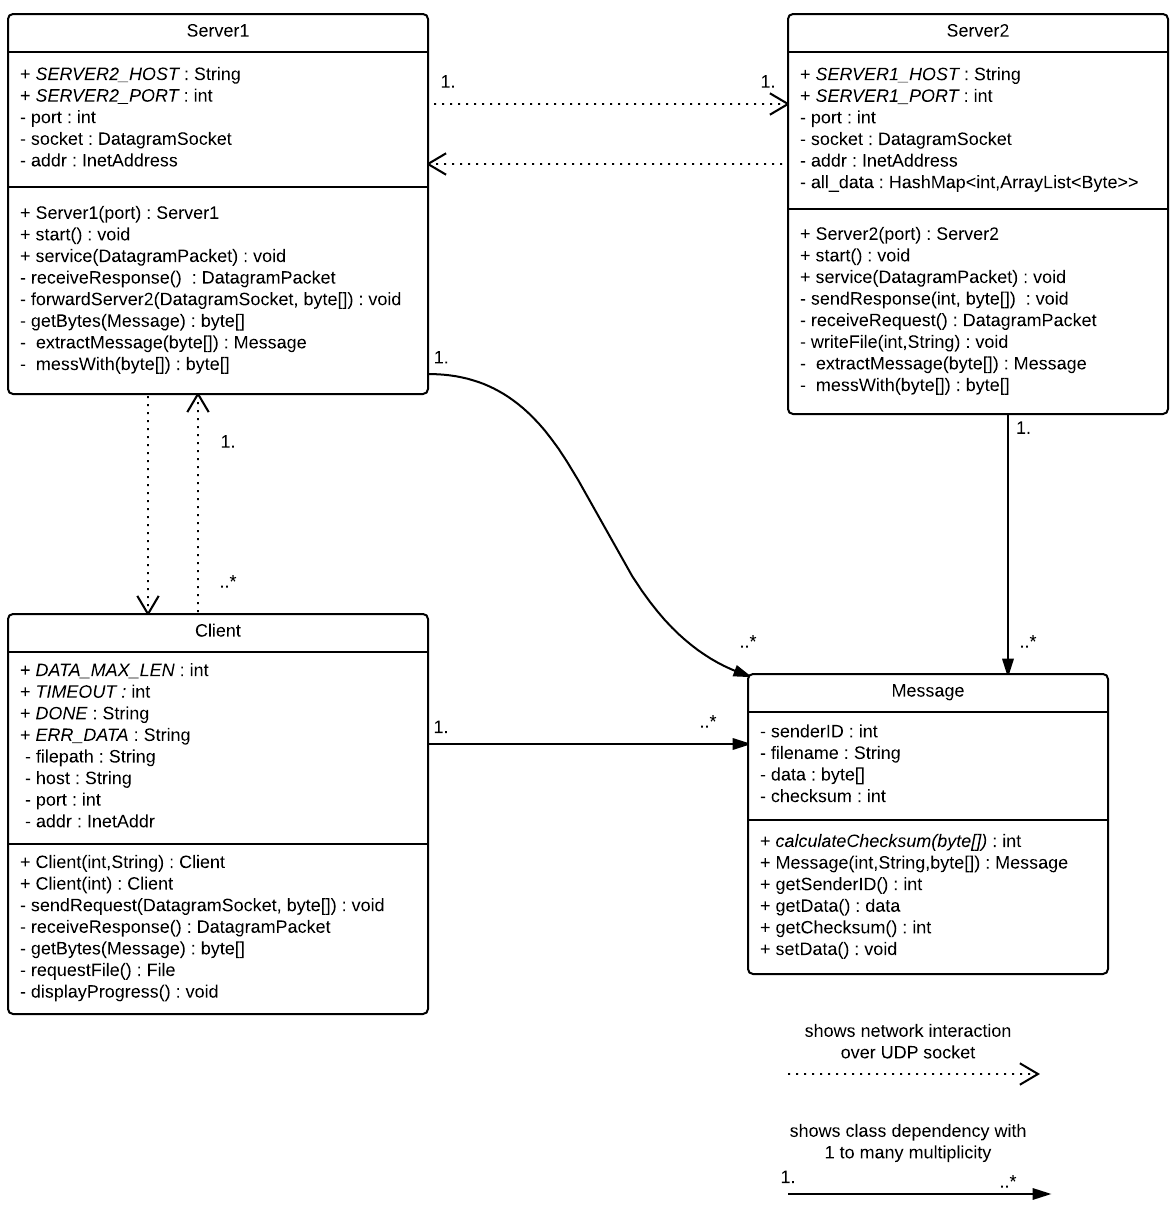
\includegraphics[width=17cm]{uml.png}
\vspace{5mm}


\end{document}
